\section{Discussion}
\label{sec:discussion}
%Strengths: Goal-prio (yay),
%Only 1 agent at a time: Weakness in solution length but strength in performance
%TODO: Mention possible impovement on Multi Agent tracks, gained from sending all commands at once. Include remarks on possible issues with this approach as well. I.e. in a level with 2 angents and 100 steps, the acutal steps could be 50, provided that no new issues arises.

This section presents some of the pros and cons of our client.
For instance we will discuss the con of only moving one agent at a time and the difference between online and offline planning.

\subsection{On Multi-agent Movement}
Our solution only sends commands to one agent at a time.
This increases the length of results in multi-agent levels but it also give us better performance.
By performance we mean the time spent to find a solution (from starting the client to the server responds with \texttt{success}).
By only moving one agent at a time we do not have to look for conflicts between the agents' paths but simply move obstacles.
The simplicity of our client was advantageous while competing against the other group's more complicated solutions.
It was clear that we could out-perform them in time spent on finding a solution.

Of course, if the client could move multiple agents simultaneously, this would have been a great improvement on number of actions performed.
For example consider \cref{fig:intuition example} again, if all agents moved at the same time then all the blocking boxes would be moved out of the way simultaneously.
But by moving all agents simultaneously we would risk getting conflicts if two or more agents' paths crossed.
To solve these conflicts we could either do offline planning and make a complete plan before execution.
This would hurt our solving times on multi-agent levels since we would have to cross check all paths.
We could also try to solve the conflicts as they come in our online planning.
This way we would solve conflicts as we go, but we risk live-locks if two agents get stuck in each others paths.
We would be forced to handle these challenges, which would most likely decrease our client's performance.

A third option is to inspect if multiple paths cross, and simultaneously execute them if they are disjoint.
Otherwise, the path without dependencies should move first, and the others that cross the original path must wait.
This way it would most likely only hurt our performance a little, but the number of actions would not be improved a lot and only on some levels.

%\emph{What are the strengths and weaknesses of your solution? Why did you choose your particular solution method, and did it work out as expected? If it didn’t work as expected, what should have been different? Here you can also include a deeper comparative analysis if you have implemented different methods/clients. Which worked best? Can you get better than that? How?}
%
We decided to do goal prioritisation over agent prioritisation because we wanted to solve the inner most goals if goals would block for each other.
Our goal prioritisation makes sure that we in most cases do not solve a goal if it will block for a unsolved goal.
If we had prioritisation on agents we could have gotten shorter solutions in some levels where an agent start close to a box and goal but it chooses another goal that is further away because that goal has a higher priority.
Our solution gives us less conflicts and less moving of boxes on solve goals.


\subsection{Goal Ordering}
\label{subsec:disc_goal_ordering}

As shown in \cref{sec:results}, our goal prioritisation algorithm enables us to solve 16 out of the 30 given solvable levels. 
It is however important in this discussion segment to stress some of the flaws that come with our algorithm. 
In this subsection we'll outline some of the strengths and weaknesses found in our goal prioritisation. 

\subsubsection{Strengths} From the competition we learned that our client was succesfully able to prioritise goals in levels such as \texttt{MAteamhal}. 
This level includes one opening which branches into two different one-way paths, as can be seen in the included \cref{fig:mateamhal}.
This can be attributed to the fact that our ordering algorithm increments the opening of the goals (in this case the middle), for each iteration of the scoring matrix (see \cref{methods:goal_ordering}). 
As such the opening in the middle will get the heighest score, and therefore everything following will decrese. 
With this technique, we are able to solve both problems like \texttt{MAteamhal}, as well as levels with different groups of goals. 

\begin{figure}[h!]
  \centering
  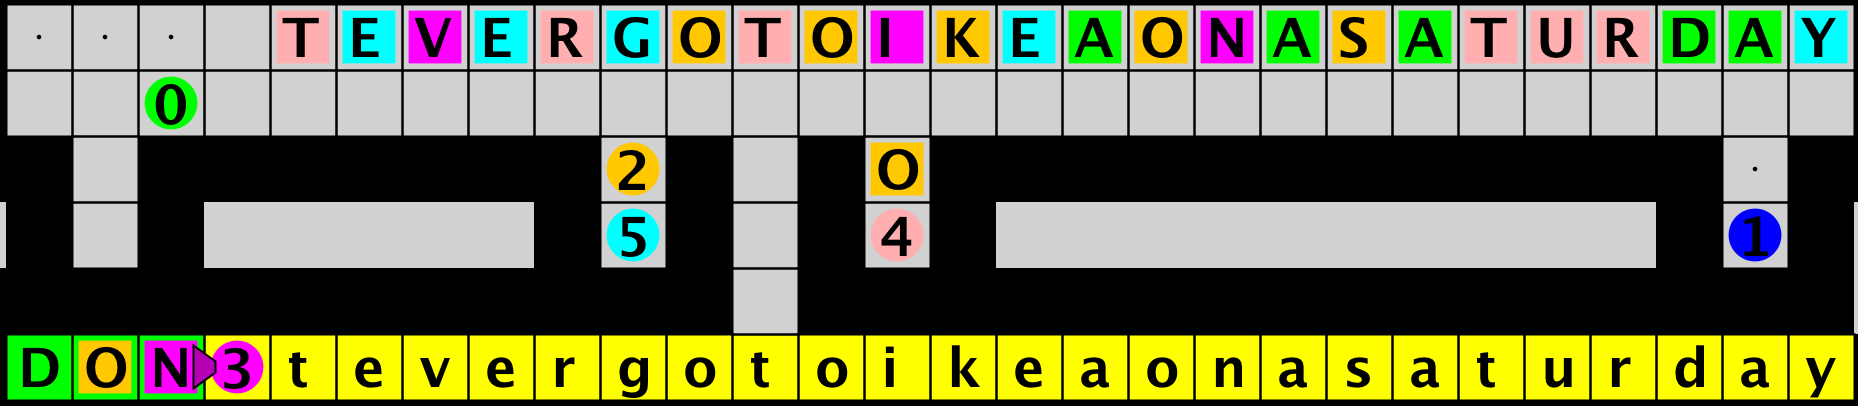
\includegraphics[width=.7\columnwidth]{graphics/mateahhal.png}
  \caption{\label{fig:mateamhal}Our client solving MAteamhal}
\end{figure}

\subsubsection{Weaknesses} Defining the opening (or entrance) to a group of goals as the goal with the most neighbouring free cells, does have it issues however. 
While working great in cases such as the one seen in \cref{fig:mateamhal}, problems arise if the entrance to a group of goals is not actually the goal with the heighest number of neighbouring free cells. 
An example of this can be found in \cref{fig:examplelev}.
Here we see that goal \textbf{c} has the heighest number of neighboring free cells, and as such, our ordering algorithm will find it to be blocking the other goals, even though it is not. 
In the class competition, we did not encounter a problem like this, however the problem is indeed a known weakness of our prioritisation algorithm.

\begin{figure}[h!]
  \centering
  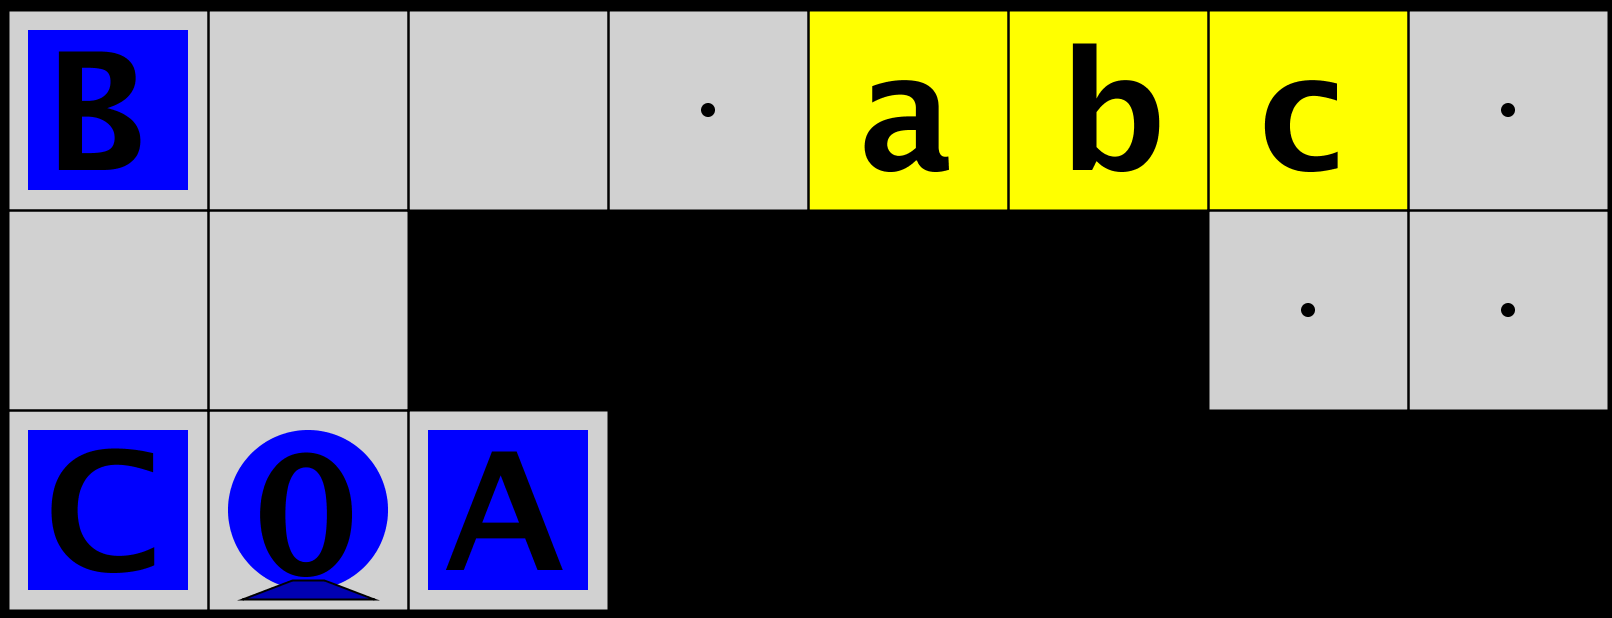
\includegraphics[width=.6\columnwidth]{graphics/ordering_issue.png}
  \caption{\label{fig:examplelev}Example level}
\end{figure}
 
\subsection{Online and Offline Planning}

Unable to look into the future because we solve sub-goals and don't build a plan for solving the entire level.

Offline planning is applicable for this domain because it is deterministic, static and fully observable.

Biggest challenge for offline planning is the combinatorial explosion/branching factor for planning for all possible contingencies for an entire plan.

More naturally online planning (and replanning) aims to achieve sub-goals that will eventually lead to a solution to the grand goal.

Furthermore, with online planning the client can plan for unseen future effects of past actions.
Note, we assumed that the domain was deterministic and fully observable for offline planning to be applicable.
By monitoring the execution of actions the client can keep and updated perception of the world in which the agents are performing actions.


\subsection{Centralised and Decentralised Planning}

Our client incorporates a single-agent multibody planner, which plans to achieve goals in a prioritised order.
Compared to a multi-agent planner, our client will never encounter conflicts with other agent's plans that need to be resolved.
On the other hand, if multiple agents could have performed actions simultaneously now they must wait for the other to finish, and thus the number of actions performed will automatically be higher.

If we consider that the planner could handle multiple agents simultaneously, then the client must be able to handle conflicts with other agents.
This would for instance be in the form of social laws, where agents consider each others identifier to decide which agent must make room for the other.
Agent's could also communicate their intentions to each other, and thereby coordinate conflict free paths.
Moreover, it could also be possible to perform some kind of agent prioritisation based on the agent's identifier or the path which the respective agent is currently moving along.
As we presented in \cref{sec:related work}, some of these ideas have been proposed in related work.

Furthermore, if multiple agents move simultaneously then it could happen that their movement would be caught in a live lock, i.e. they move in an endless loop trying to move past each other.

